\documentclass[11pt,a4paper]{article}

% --- Packages ---
\usepackage[utf8]{inputenc}
\usepackage[T1]{fontenc}
\usepackage{amsmath,amssymb,amsfonts}
\usepackage{geometry}
\usepackage{xcolor}
\usepackage{enumitem}
\usepackage{booktabs}
\usepackage{array}
\usepackage{multirow}
\usepackage{tikz}
\usepackage{graphicx}
\usepackage{fancyhdr}
\usepackage{tabularx}
\usepackage{listings}
\usepackage[normalem]{ulem} % For \dashuline (dashed underline)

\usetikzlibrary{shapes,arrows,positioning,calc,graphs,quotes}

% --- Page Geometry ---
\geometry{a4paper, margin=1in}

% --- Header/Footer Setup ---
\pagestyle{fancy}
\fancyhf{}
\fancyhead[L]{Database Systems - Practice Exam}
\fancyhead[R]{Practice Exam}
\fancyfoot[C]{\thepage}
\renewcommand{\headrulewidth}{0.4pt}

\setlength{\parskip}{6pt}
\setlength{\parindent}{0pt}

\title{\textbf{Database Systems\\Practice Examination}}
\author{}
\date{}

\begin{document}

\maketitle
\thispagestyle{empty}

\section*{Preamble}

Please read the following instructions carefully:

\begin{itemize}
\item This exam has seven questions and 13 pages. Make sure your copy contains all exercises and all questions. The following table summarizes the questions in this exam and their weights.

\begin{center}
\begin{tabular}{|l|c|}
\hline
\textbf{Question} & \textbf{Points} \\
\hline
1. Relational Algebra & 10 \\
2. SQL & 20 \\
3. ER Modeling & 16 \\
4. Design Theory & 14 \\
5. Physical Design & 12 \\
6. Query Processing and Optimization & 14 \\
7. Transactions, Concurrency Control, and Recovery & 14 \\
\hline
\textbf{Total} & \textbf{100} \\
\hline
\end{tabular}
\end{center}

\item Read the text of each exercise carefully before solving it.
\item If you get stuck on an exercise, proceed with another one and come back later.
\item If your solution is based on an assumption that you have made, please add a comment for clarification.
\item Aids are allowed during the exam, i.e., you can consult aids such as books, notes, etc.
\item As a reference, we recommend the course material (book, slides, exercises, etc.) as it complies with the notation used in the exam.
\item It is NOT allowed to seek help from or consult others (human beings, artificial intelligence, etc.) during the exam.
\item Good luck!
\end{itemize}

\newpage

\section{Relational Algebra (10 points)}

Consider the following relations capturing information about a movie streaming service:

\begin{verbatim}
studio(sid, studioName, country, foundedYear)
movie(mid, title, genre, releaseYear, sid -> studio)
subscriber(uid, username, email, subscription)
viewing(uid -> subscriber, mid -> movie, watchDate, rating)
\end{verbatim}

where the primary keys are underlined and the foreign keys are denoted by arrows.

Fill in the missing information that should go into the boxes to make the query compute the required information. Note that your solution should not output additional information.

To enter the operation symbols into the answer sheet, please use the following replacements:

\begin{center}
\begin{tabular}{|l|l|}
\hline
\textbf{Operation symbol} & \textbf{What to write in the answer sheet} \\
\hline
$\rho$ & rho \\
$\gamma$ & gamma \\
$\Pi$ & pi \\
$\sigma$ & sigma \\
$\bowtie$ & join \\
$\times$ & x \\
$-$ & minus \\
\hline
\end{tabular}
\end{center}

\subsection{(4 points)}
Find all subscribers who have watched movies from studios in 'USA' and gave a rating of 5. For each such subscriber, list their uid and username.

\begin{center}
\fbox{Box 1}\textsubscript{uid, username} (\fbox{Box 2}\textsubscript{rating = 5} (subscriber $\bowtie$ viewing $\bowtie$ movie $\bowtie$ (\fbox{Box 3}\textsubscript{country = 'USA'} (\fbox{Box 4}))))
\end{center}

\vspace{1em}

\subsection{(6 points)}
Find all subscribers who have NOT watched any Horror movie. For each such subscriber, list their uid.

\begin{center}
$\Pi_{\text{uid}}$(\fbox{Box 5}) \fbox{Box 6} $\Pi_{\text{uid}}$(viewing $\bowtie_{\text{viewing.mid = movie.mid}}$ (\fbox{Box 7}\textsubscript{genre = 'Horror'} (\fbox{Box 8})))
\end{center}

\newpage

\section{SQL (20 points)}

\subsection{Evaluate whether the following statements about SQL are true or false.}

\subsubsection{(2 points)}
The expression \texttt{NULL = NULL} evaluates to TRUE in SQL.

(a) True \quad\quad (b) False

\subsubsection{(2 points)}
The condition \texttt{x IN (empty set)} evaluates to FALSE, while \texttt{x > ALL (empty set)} evaluates to TRUE.

(a) True \quad\quad (b) False

\subsection{Consider again the relational schema from Question 1:}

\begin{verbatim}
studio(sid, studioName, country, foundedYear)
movie(mid, title, genre, releaseYear, sid -> studio)
subscriber(uid, username, email, subscription)
viewing(uid -> subscriber, mid -> movie, watchDate, rating)
\end{verbatim}

where the primary keys are underlined and the foreign keys are denoted by arrows.

Answer the following questions:

\subsubsection{(4 points)}
Which of the following queries correctly finds the average rating per movie genre? For each genre, list the genre and the average. Choose \textbf{only one} option:

(a) SELECT genre, AVG(rating)\\
\phantom{xxxx}FROM viewing, movie\\
\phantom{xxxx}GROUP BY genre;

(b) SELECT m.genre, AVG(v.rating)\\
\phantom{xxxx}FROM viewing v JOIN movie m ON v.mid = m.mid\\
\phantom{xxxx}GROUP BY m.genre;

(c) SELECT genre, AVG(rating)\\
\phantom{xxxx}FROM viewing\\
\phantom{xxxx}GROUP BY genre;

(d) SELECT AVG(rating)\\
\phantom{xxxx}FROM viewing, movie\\
\phantom{xxxx}WHERE genre GROUP BY genre;

(e) Both (a) and (b) are correct.

(f) None of the above

\subsubsection{(4 points)}
Which of the following queries correctly finds subscribers who have watched more than 10 movies? For each such subscriber, list their uid and the count. Choose \textbf{only one} option:

(a) SELECT uid, COUNT(*)\\
\phantom{xxxx}FROM viewing\\
\phantom{xxxx}WHERE COUNT(*) > 10\\
\phantom{xxxx}GROUP BY uid;

(b) SELECT uid, COUNT(*)\\
\phantom{xxxx}FROM viewing\\
\phantom{xxxx}GROUP BY uid\\
\phantom{xxxx}HAVING COUNT(*) > 10;

(c) SELECT uid\\
\phantom{xxxx}FROM viewing\\
\phantom{xxxx}GROUP BY uid\\
\phantom{xxxx}HAVING mid > 10;

(d) SELECT uid\\
\phantom{xxxx}FROM viewing\\
\phantom{xxxx}HAVING COUNT(*) > 10;

(e) Both (a) and (b) are correct.

(f) None of the above

\subsubsection{(4 points)}
Fill in the missing information that should go into the boxes of the following query: find all studios that have at least one Action movie. For each such studio, list sid and studioName.

\begin{verbatim}
SELECT DISTINCT s.sid, s.studioName
FROM studio s
WHERE [Box 1] (
    SELECT * FROM movie m
    WHERE m.sid = s.sid [Box 2] m.genre = 'Action'
);
\end{verbatim}

\subsubsection{(4 points)}
Consider the following query that finds subscribers who have never watched any movie:

\begin{verbatim}
SELECT s.uid, s.username
FROM subscriber s LEFT JOIN viewing v ON s.uid = v.uid
WHERE v.uid IS NULL;
\end{verbatim}

Which of the following statements is \textbf{correct}? Choose \textbf{one or more} options:

(a) This query uses an outer join to preserve all subscribers.

(b) The WHERE clause filters for subscribers with no matching viewing records.

(c) This query is equivalent to: \texttt{SELECT uid, username FROM subscriber WHERE uid NOT IN (SELECT uid FROM viewing)}.

(d) If we replace LEFT JOIN with INNER JOIN, the query would return an empty result set (no rows).

(e) The condition \texttt{v.uid IS NULL} checks for subscribers without any viewings.

(f) All of the above.

\newpage

\section{ER Modeling (16 points)}

\subsection{Evaluate whether the following statements about ER model concepts are true or false.}

\subsubsection{(2 points)}
A weak entity type is represented by a double-bordered rectangle and its identifying relationship by a double-bordered diamond.

(a) True \quad\quad (b) False

\subsubsection{(2 points)}
When mapping a 1:N relationship to the relational model, the foreign key is placed on the ``one'' side of the relationship.

(a) True \quad\quad (b) False

\subsubsection{(2 points)}
A composite attribute should be flattened to its simple component attributes when mapping to the relational model (the composite attribute itself is not stored).

(a) True \quad\quad (b) False

\subsection{(4 points)}
Consider the relationship \textit{reserves} where
\begin{itemize}
\item each \textit{room} can be reserved by many guests or no guest (partial participation)
\item each \textit{guest} must reserve at least one room (total participation)
\end{itemize}

Which of the following ER diagram representations is \textbf{correct}? Choose \textbf{only one} option:

\textit{Note: Chen notation (1, N, M) is placed near the relationship diamond. [min, max] notation is placed near the entity. Double lines indicate total participation.}

\begin{center}
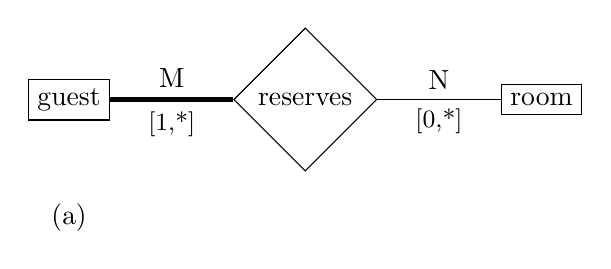
\begin{tikzpicture}[node distance=3cm]
\node[draw, rectangle] (g) {guest};
\node[draw, diamond, right of=g, node distance=3cm] (r) {reserves};
\node[draw, rectangle, right of=r, node distance=3cm] (rm) {room};
\draw[line width=2pt] (g) -- node[above] {M} node[below] {\small [1,*]} (r);
\draw (r) -- node[above] {N} node[below] {\small [0,*]} (rm);
\node[below of=g, node distance=1.5cm] {(a)};
\end{tikzpicture}
\end{center}

\begin{center}
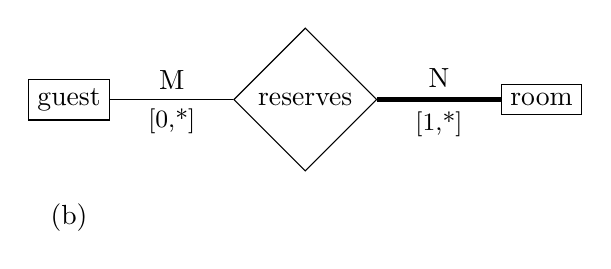
\begin{tikzpicture}[node distance=3cm]
\node[draw, rectangle] (g) {guest};
\node[draw, diamond, right of=g, node distance=3cm] (r) {reserves};
\node[draw, rectangle, right of=r, node distance=3cm] (rm) {room};
\draw (g) -- node[above] {M} node[below] {\small [0,*]} (r);
\draw[line width=2pt] (r) -- node[above] {N} node[below] {\small [1,*]} (rm);
\node[below of=g, node distance=1.5cm] {(b)};
\end{tikzpicture}
\end{center}

\begin{center}
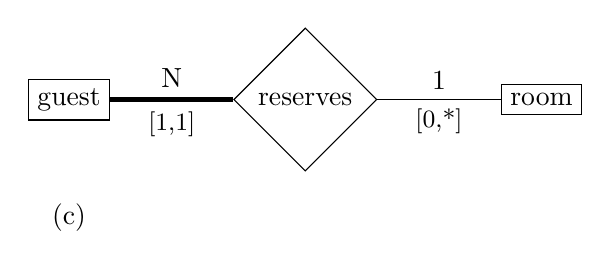
\begin{tikzpicture}[node distance=3cm]
\node[draw, rectangle] (g) {guest};
\node[draw, diamond, right of=g, node distance=3cm] (r) {reserves};
\node[draw, rectangle, right of=r, node distance=3cm] (rm) {room};
\draw[line width=2pt] (g) -- node[above] {N} node[below] {\small [1,1]} (r);
\draw (r) -- node[above] {1} node[below] {\small [0,*]} (rm);
\node[below of=g, node distance=1.5cm] {(c)};
\end{tikzpicture}
\end{center}

\begin{center}
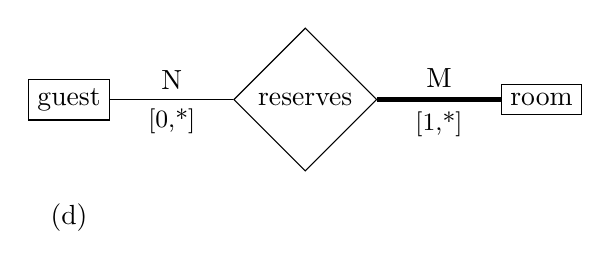
\begin{tikzpicture}[node distance=3cm]
\node[draw, rectangle] (g) {guest};
\node[draw, diamond, right of=g, node distance=3cm] (r) {reserves};
\node[draw, rectangle, right of=r, node distance=3cm] (rm) {room};
\draw (g) -- node[above] {N} node[below] {\small [0,*]} (r);
\draw[line width=2pt] (r) -- node[above] {M} node[below] {\small [1,*]} (rm);
\node[below of=g, node distance=1.5cm] {(d)};
\end{tikzpicture}
\end{center}

(e) None of the above

\subsection{(6 points)}
Consider the following ER diagram showing a music database with \textit{album} (strong entity) and \textit{song} (weak entity):

\begin{center}
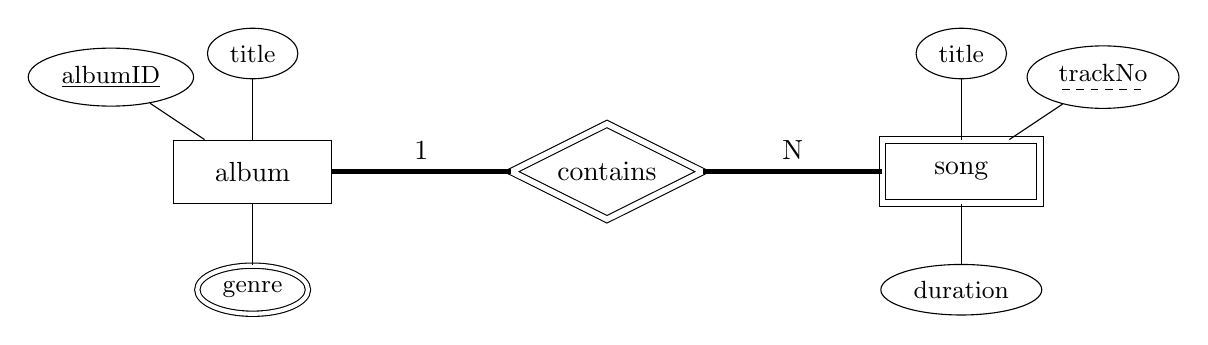
\begin{tikzpicture}[
    entity/.style={draw, rectangle, minimum width=2cm, minimum height=0.8cm},
    weakentity/.style={draw, double, rectangle, minimum width=2cm, minimum height=0.8cm, double distance=2pt},
    relationship/.style={draw, diamond, aspect=2, minimum width=1.2cm},
    weakrel/.style={draw, double, diamond, aspect=2, minimum width=1.2cm, double distance=2pt},
    attribute/.style={draw, ellipse, font=\small},
    partialkey/.style={draw, ellipse, font=\small},
    multiattr/.style={draw, ellipse, double, double distance=1.5pt, font=\small}
]
% Entities
\node[entity] (album) at (0,0) {album};
\node[weakrel] (contains) at (4.5,0) {contains};
\node[weakentity] (song) at (9,0) {song};

% Connection with Chen notation
\draw[line width=2pt] (album) -- node[above] {1} (contains);
\draw[line width=2pt] (contains) -- node[above] {N} (song);

% Album attributes
\node[attribute] (albumid) at (-1.8, 1.2) {\underline{albumID}};
\node[attribute] (albumtitle) at (0, 1.5) {title};
\node[multiattr] (genre) at (0, -1.5) {genre};
\draw (album) -- (albumid);
\draw (album) -- (albumtitle);
\draw (album) -- (genre);

% Song attributes (trackNo is partial key - dashed underline)
\node[partialkey] (trackno) at (10.8, 1.2) {\dashuline{trackNo}};
\node[attribute] (songtitle) at (9, 1.5) {title};
\node[attribute] (duration) at (9, -1.5) {duration};
\draw (song) -- (trackno);
\draw (song) -- (songtitle);
\draw (song) -- (duration);
\end{tikzpicture}
\end{center}

\textit{Note: Double rectangle = weak entity. Double diamond = identifying relationship. Dashed underline on trackNo = partial key. Double ellipse on genre = multi-valued attribute. The song entity cannot exist without its owning album.}

Which combination of relations should be created for this ER diagram? Note that we aim for a minimal schema. Choose \textbf{one or more} options:

(a) album(\underline{albumID}, title, genre)

(b) album(\underline{albumID}, title)

(c) genre(\underline{albumID $\rightarrow$ album, genreName})

(d) song(\underline{trackNo}, title, duration, albumID $\rightarrow$ album)

(e) song(\underline{albumID $\rightarrow$ album, trackNo}, title, duration)

(f) contains(\underline{albumID $\rightarrow$ album, trackNo $\rightarrow$ song})

(g) song(\underline{songID}, trackNo, title, duration, albumID $\rightarrow$ album)

(h) None of the above

\newpage

\section{Design Theory (14 points)}

\subsection{Evaluate whether the following statements about design theory are true or false.}

\subsubsection{(2 points)}
If $X \rightarrow Y$ and $Y \rightarrow Z$ are functional dependencies in $F$, then $X \rightarrow Z$ can be derived using Armstrong's axiom of transitivity.

(a) True \quad\quad (b) False

\subsubsection{(2 points)}
A relation is in BCNF if and only if every non-trivial functional dependency has a superkey on the left-hand side.

(a) True \quad\quad (b) False

\subsection{Consider a relation schema $R = (A, B, C, D, E)$ with the following functional dependencies (FDs):}

\begin{align*}
A &\rightarrow B \\
BC &\rightarrow D \\
D &\rightarrow E \\
E &\rightarrow A
\end{align*}

Answer the following questions:

\subsubsection{(4 points)}
Which of the following are \textbf{candidate keys} of $R$? Choose \textbf{one or more} options:

(a) A

(b) C

(c) AC

(d) BC

(e) DC

(f) EC

(g) ABC

(h) None of the above

\subsubsection{(3 points)}
Which of the following statements is correct about the normalization status of relation $R$? Choose \textbf{only one} option:

(a) The relation $R$ is in BCNF.

(b) The relation $R$ is in 3NF but not in BCNF.

(c) The relation $R$ is in 2NF but not in 3NF.

(d) The relation $R$ is not in 2NF.

(e) None of the above

\subsubsection{(3 points)}
Which of the following decompositions of the relational schema $R = (A, B, C, D, E)$ is \textbf{lossless}? Choose \textbf{one or more} options:

(a) $R_1 = (A, B, C)$ and $R_2 = (C, D, E)$

(b) $R_1 = (A, B, D)$ and $R_2 = (D, E, C)$

(c) $R_1 = (B, C, D)$ and $R_2 = (A, D, E)$

(d) $R_1 = (A, B)$ and $R_2 = (B, C, D, E)$

(e) None of the above

\newpage

\section{Physical Design (12 points)}

\subsection{Evaluate whether the following statements about B+ Trees are true or false.}

\subsubsection{(2 points)}
In a B+ Tree, all data records (or pointers to data records) are stored only in the leaf nodes, while internal nodes contain only keys and child pointers.

(a) True \quad\quad (b) False

\subsubsection{(2 points)}
For a B+ Tree with degree $d = 5$, a leaf node must contain at least 2 keys.

(a) True \quad\quad (b) False

\subsection{Consider the following B+ Tree with degree $d = 4$.}

\begin{center}
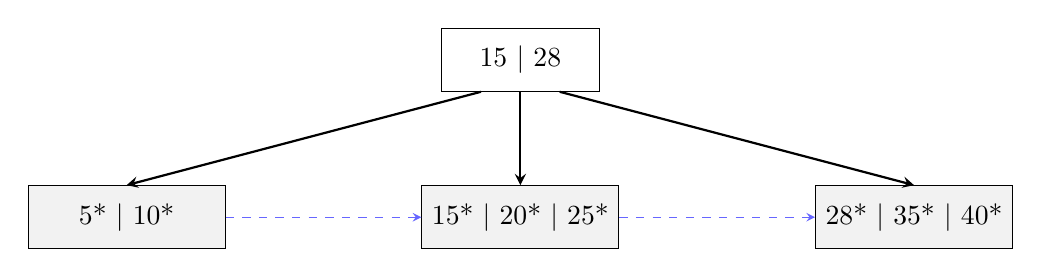
\begin{tikzpicture}[
  bptree/.style={draw, rectangle, minimum height=0.8cm, font=\normalsize},
  internal/.style={bptree, minimum width=2cm},
  leaf/.style={bptree, minimum width=2.5cm, fill=gray!10},
  ptr/.style={->, >=stealth, thick},
  sibling/.style={->, >=stealth, dashed, blue!60}
]
% Root
\node[internal] (root) at (0,0) {15 $|$ 28};

% Level 1 - Leaf nodes (d=4: max 3 keys, min 2 keys per leaf)
\node[leaf] (leaf1) at (-5,-2) {5* $|$ 10*};
\node[leaf] (leaf2) at (0,-2) {15* $|$ 20* $|$ 25*};
\node[leaf] (leaf3) at (5,-2) {28* $|$ 35* $|$ 40*};

% Root to leaf pointers
\draw[ptr] (root.south) ++(-0.5,0) -- (leaf1.north);
\draw[ptr] (root.south) -- (leaf2.north);
\draw[ptr] (root.south) ++(0.5,0) -- (leaf3.north);

% Sibling pointers between leaves
\draw[sibling] (leaf1.east) -- (leaf2.west);
\draw[sibling] (leaf2.east) -- (leaf3.west);
\end{tikzpicture}
\end{center}

Please make the following assumptions:
\begin{itemize}
\item The left pointer of a key $k$ in a non-leaf node leads towards keys less than $k$, while the right pointer leads towards keys greater than or equal to $k$.
\item A leaf node underflows when the number of keys goes below $\lceil \frac{d-1}{2} \rceil$.
\item An internal node underflows when the number of pointers goes below $\lceil \frac{d}{2} \rceil$.
\end{itemize}

Answer the following questions:

\subsubsection{(4 points)}
Delete 5*, then delete 10*. What is the resulting tree? Choose \textbf{only one} option:

\vspace{1em}
\noindent
(a)
\begin{center}
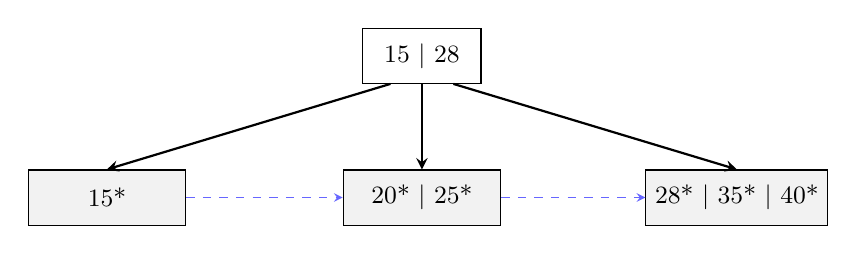
\begin{tikzpicture}[
  bptree/.style={draw, rectangle, minimum height=0.7cm, font=\small},
  internal/.style={bptree, minimum width=1.5cm},
  leaf/.style={bptree, minimum width=2cm, fill=gray!10},
  ptr/.style={->, >=stealth, thick},
  sibling/.style={->, >=stealth, dashed, blue!60}
]
\node[internal] (root) at (0,0) {15 $|$ 28};
\node[leaf] (l1) at (-4,-1.8) {15*};
\node[leaf] (l2) at (0,-1.8) {20* $|$ 25*};
\node[leaf] (l3) at (4,-1.8) {28* $|$ 35* $|$ 40*};
\draw[ptr] (root.south) ++(-0.4,0) -- (l1.north);
\draw[ptr] (root.south) -- (l2.north);
\draw[ptr] (root.south) ++(0.4,0) -- (l3.north);
\draw[sibling] (l1.east) -- (l2.west);
\draw[sibling] (l2.east) -- (l3.west);
\end{tikzpicture}
\end{center}

\vspace{1em}
\noindent
(b)
\begin{center}
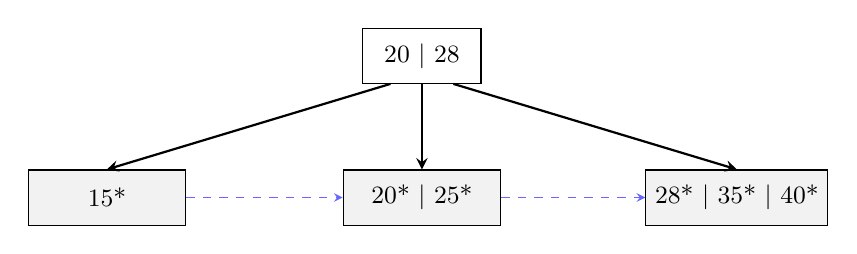
\begin{tikzpicture}[
  bptree/.style={draw, rectangle, minimum height=0.7cm, font=\small},
  internal/.style={bptree, minimum width=1.5cm},
  leaf/.style={bptree, minimum width=2cm, fill=gray!10},
  ptr/.style={->, >=stealth, thick},
  sibling/.style={->, >=stealth, dashed, blue!60}
]
\node[internal] (root) at (0,0) {20 $|$ 28};
\node[leaf] (l1) at (-4,-1.8) {15*};
\node[leaf] (l2) at (0,-1.8) {20* $|$ 25*};
\node[leaf] (l3) at (4,-1.8) {28* $|$ 35* $|$ 40*};
\draw[ptr] (root.south) ++(-0.4,0) -- (l1.north);
\draw[ptr] (root.south) -- (l2.north);
\draw[ptr] (root.south) ++(0.4,0) -- (l3.north);
\draw[sibling] (l1.east) -- (l2.west);
\draw[sibling] (l2.east) -- (l3.west);
\end{tikzpicture}
\end{center}

\vspace{1em}
\noindent
(c)
\begin{center}
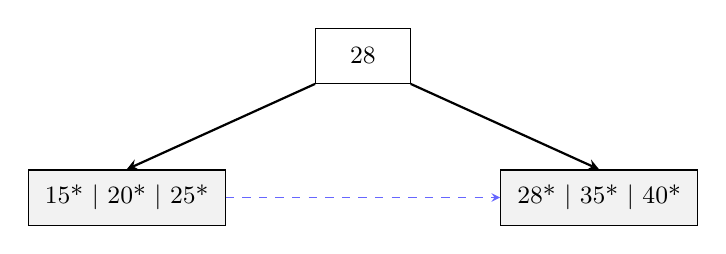
\begin{tikzpicture}[
  bptree/.style={draw, rectangle, minimum height=0.7cm, font=\small},
  internal/.style={bptree, minimum width=1.2cm},
  leaf/.style={bptree, minimum width=2.5cm, fill=gray!10},
  ptr/.style={->, >=stealth, thick},
  sibling/.style={->, >=stealth, dashed, blue!60}
]
\node[internal] (root) at (0,0) {28};
\node[leaf] (l1) at (-3,-1.8) {15* $|$ 20* $|$ 25*};
\node[leaf] (l2) at (3,-1.8) {28* $|$ 35* $|$ 40*};
\draw[ptr] (root.south west) -- (l1.north);
\draw[ptr] (root.south east) -- (l2.north);
\draw[sibling] (l1.east) -- (l2.west);
\end{tikzpicture}
\end{center}

\vspace{1em}
\noindent
(d)
\begin{center}
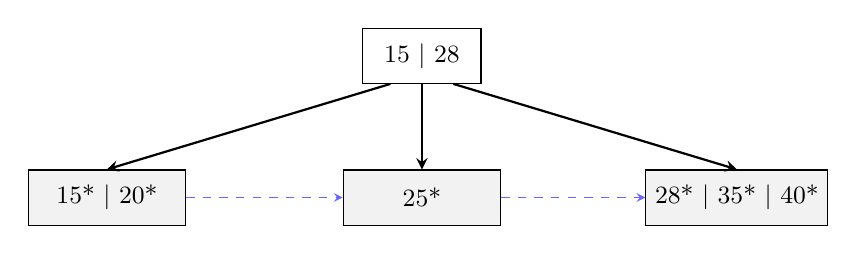
\begin{tikzpicture}[
  bptree/.style={draw, rectangle, minimum height=0.7cm, font=\small},
  internal/.style={bptree, minimum width=1.5cm},
  leaf/.style={bptree, minimum width=2cm, fill=gray!10},
  ptr/.style={->, >=stealth, thick},
  sibling/.style={->, >=stealth, dashed, blue!60}
]
\node[internal] (root) at (0,0) {15 $|$ 28};
\node[leaf] (l1) at (-4,-1.8) {15* $|$ 20*};
\node[leaf] (l2) at (0,-1.8) {25*};
\node[leaf] (l3) at (4,-1.8) {28* $|$ 35* $|$ 40*};
\draw[ptr] (root.south) ++(-0.4,0) -- (l1.north);
\draw[ptr] (root.south) -- (l2.north);
\draw[ptr] (root.south) ++(0.4,0) -- (l3.north);
\draw[sibling] (l1.east) -- (l2.west);
\draw[sibling] (l2.east) -- (l3.west);
\end{tikzpicture}
\end{center}

\vspace{0.5em}
(e) None of the above

\subsubsection{(4 points)}
Consider the original tree (ignore operations in 5.2.1). Insert 22* into the tree. What is the resulting tree? Choose \textbf{only one} option:

\vspace{1em}
\noindent
(a)
\begin{center}
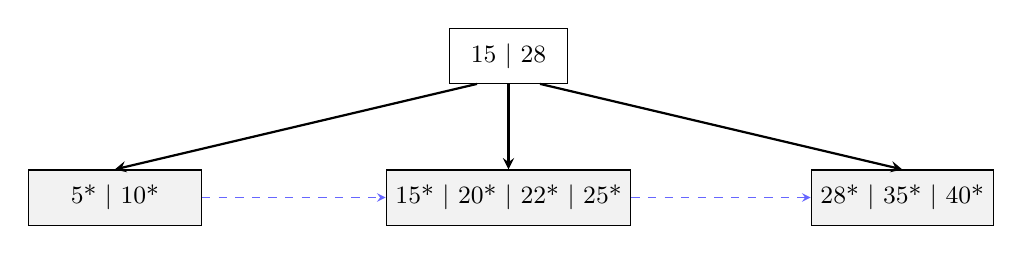
\begin{tikzpicture}[
  bptree/.style={draw, rectangle, minimum height=0.7cm, font=\small},
  internal/.style={bptree, minimum width=1.5cm},
  leaf/.style={bptree, minimum width=2.2cm, fill=gray!10},
  ptr/.style={->, >=stealth, thick},
  sibling/.style={->, >=stealth, dashed, blue!60}
]
\node[internal] (root) at (0,0) {15 $|$ 28};
\node[leaf] (l1) at (-5,-1.8) {5* $|$ 10*};
\node[leaf] (l2) at (0,-1.8) {15* $|$ 20* $|$ 22* $|$ 25*};
\node[leaf] (l3) at (5,-1.8) {28* $|$ 35* $|$ 40*};
\draw[ptr] (root.south) ++(-0.4,0) -- (l1.north);
\draw[ptr] (root.south) -- (l2.north);
\draw[ptr] (root.south) ++(0.4,0) -- (l3.north);
\draw[sibling] (l1.east) -- (l2.west);
\draw[sibling] (l2.east) -- (l3.west);
\end{tikzpicture}
\end{center}

\vspace{1em}
\noindent
(b)
\begin{center}
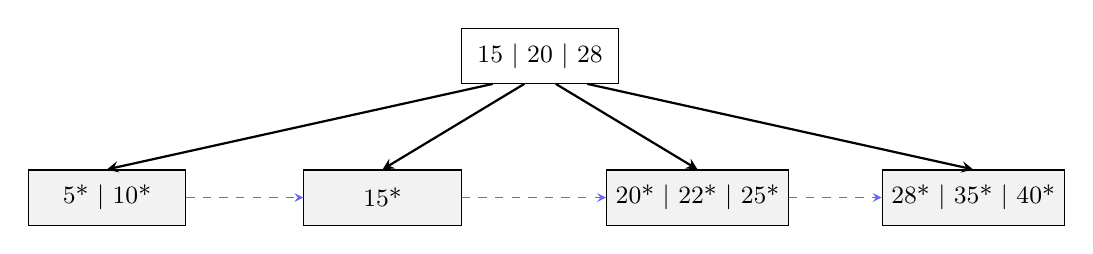
\begin{tikzpicture}[
  bptree/.style={draw, rectangle, minimum height=0.7cm, font=\small},
  internal/.style={bptree, minimum width=2cm},
  leaf/.style={bptree, minimum width=2cm, fill=gray!10},
  ptr/.style={->, >=stealth, thick},
  sibling/.style={->, >=stealth, dashed, blue!60}
]
\node[internal] (root) at (0,0) {15 $|$ 20 $|$ 28};
\node[leaf] (l1) at (-5.5,-1.8) {5* $|$ 10*};
\node[leaf] (l2) at (-2,-1.8) {15*};
\node[leaf] (l3) at (2,-1.8) {20* $|$ 22* $|$ 25*};
\node[leaf] (l4) at (5.5,-1.8) {28* $|$ 35* $|$ 40*};
\draw[ptr] (root.south) ++(-0.6,0) -- (l1.north);
\draw[ptr] (root.south) ++(-0.2,0) -- (l2.north);
\draw[ptr] (root.south) ++(0.2,0) -- (l3.north);
\draw[ptr] (root.south) ++(0.6,0) -- (l4.north);
\draw[sibling] (l1.east) -- (l2.west);
\draw[sibling] (l2.east) -- (l3.west);
\draw[sibling] (l3.east) -- (l4.west);
\end{tikzpicture}
\end{center}

\vspace{1em}
\noindent
(c)
\begin{center}
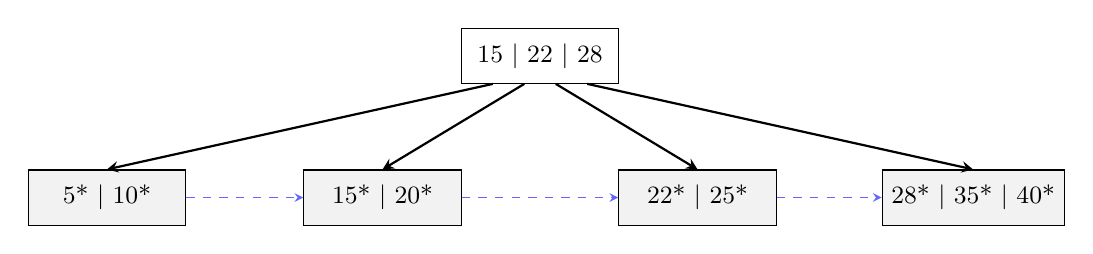
\begin{tikzpicture}[
  bptree/.style={draw, rectangle, minimum height=0.7cm, font=\small},
  internal/.style={bptree, minimum width=2cm},
  leaf/.style={bptree, minimum width=2cm, fill=gray!10},
  ptr/.style={->, >=stealth, thick},
  sibling/.style={->, >=stealth, dashed, blue!60}
]
\node[internal] (root) at (0,0) {15 $|$ 22 $|$ 28};
\node[leaf] (l1) at (-5.5,-1.8) {5* $|$ 10*};
\node[leaf] (l2) at (-2,-1.8) {15* $|$ 20*};
\node[leaf] (l3) at (2,-1.8) {22* $|$ 25*};
\node[leaf] (l4) at (5.5,-1.8) {28* $|$ 35* $|$ 40*};
\draw[ptr] (root.south) ++(-0.6,0) -- (l1.north);
\draw[ptr] (root.south) ++(-0.2,0) -- (l2.north);
\draw[ptr] (root.south) ++(0.2,0) -- (l3.north);
\draw[ptr] (root.south) ++(0.6,0) -- (l4.north);
\draw[sibling] (l1.east) -- (l2.west);
\draw[sibling] (l2.east) -- (l3.west);
\draw[sibling] (l3.east) -- (l4.west);
\end{tikzpicture}
\end{center}

\vspace{1em}
\noindent
(d)
\begin{center}
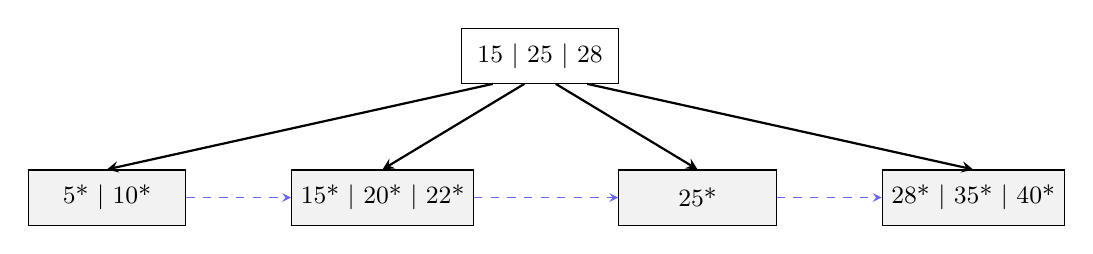
\begin{tikzpicture}[
  bptree/.style={draw, rectangle, minimum height=0.7cm, font=\small},
  internal/.style={bptree, minimum width=2cm},
  leaf/.style={bptree, minimum width=2cm, fill=gray!10},
  ptr/.style={->, >=stealth, thick},
  sibling/.style={->, >=stealth, dashed, blue!60}
]
\node[internal] (root) at (0,0) {15 $|$ 25 $|$ 28};
\node[leaf] (l1) at (-5.5,-1.8) {5* $|$ 10*};
\node[leaf] (l2) at (-2,-1.8) {15* $|$ 20* $|$ 22*};
\node[leaf] (l3) at (2,-1.8) {25*};
\node[leaf] (l4) at (5.5,-1.8) {28* $|$ 35* $|$ 40*};
\draw[ptr] (root.south) ++(-0.6,0) -- (l1.north);
\draw[ptr] (root.south) ++(-0.2,0) -- (l2.north);
\draw[ptr] (root.south) ++(0.2,0) -- (l3.north);
\draw[ptr] (root.south) ++(0.6,0) -- (l4.north);
\draw[sibling] (l1.east) -- (l2.west);
\draw[sibling] (l2.east) -- (l3.west);
\draw[sibling] (l3.east) -- (l4.west);
\end{tikzpicture}
\end{center}

\vspace{0.5em}
(e) None of the above

\newpage

\section{Query Processing and Optimization (14 points)}

\subsection{Evaluate whether the following statements about external sorting are true or false.}

\subsubsection{(2 points)}
In 2-Way External Merge Sort, Phase 1 reads one page at a time, sorts it in memory, and writes it back to disk---producing $N$ sorted runs of 1 page each from an input file of $N$ pages.

(a) True \quad\quad (b) False

\subsubsection{(2 points)}
In Multi-Way External Merge Sort with $B$ buffer pages, Phase 1 reads $B$ pages at a time, sorts them in memory, and writes out sorted runs of $B$ pages each.

(a) True \quad\quad (b) False

\subsection{Consider a database with relation $R$ containing 80,000 tuples, where 40 tuples fit on one page. The system has 101 buffer pages available.}

Answer the following questions:

\subsubsection{(4 points)}
Suppose you need to sort relation $R$ using Multi-Way External Merge Sort. Which of the following statements is \textbf{correct}? Choose \textbf{one or more} options:

(a) The number of pages for $R$ is 2,000.

(b) Phase 1 creates $\lceil 2000/101 \rceil = 20$ initial sorted runs.

(c) Phase 2 can merge up to 100 runs per pass (using $B-1$ input buffers and 1 output buffer).

(d) Since $20 < 100$, Phase 2 requires only 1 pass.

(e) The total I/O cost is $2 \times 2000 \times 2 = 8,000$ page I/Os.

(f) None of the above

\subsubsection{(2 points)}
For the same relation $R$ (2,000 pages), if we use 2-Way External Merge Sort instead, the number of passes in Phase 2 would be $\lceil \log_2 N \rceil$ where $N$ is the number of initial runs. Since 2-Way Sort creates $N = 2000$ initial runs (one per page), how many passes are needed in Phase 2? Choose \textbf{only one} option:

(a) 10 passes

(b) 11 passes

(c) 20 passes

(d) 2000 passes

(e) None of the above

\subsection{(4 points)}
Consider two relations: $R$ has 1,000 pages and $S$ has 500 pages. Each page has 100 tuples. The system has 102 buffer pages available. You need to join $R$ and $S$ using Block Nested-Loop Join.

Which of the following statements is \textbf{correct}? Choose \textbf{one or more} options:

(a) Using $S$ as the outer relation: Cost = $500 + \lceil 500/100 \rceil \times 1000 = 500 + 5 \times 1000 = 5,500$ page I/Os.

(b) Using $R$ as the outer relation: Cost = $1000 + \lceil 1000/100 \rceil \times 500 = 1000 + 10 \times 500 = 6,000$ page I/Os.

(c) The smaller relation ($S$) should be used as the outer relation to minimize I/O cost.

(d) In Block Nested-Loop Join, $(B-2)$ pages are used for the outer relation block, 1 page for scanning the inner relation, and 1 page for output.

(e) If we used Page-Oriented Nested-Loop Join instead with $R$ as outer, the cost would be $1000 + 1000 \times 500 = 501,000$ page I/Os.

(f) None of the above

\newpage

\section{Transactions, Concurrency Control, and Recovery (14 points)}

\subsection{Evaluate whether the following statements are true or false.}

\subsubsection{(2 points)}
The REDO phase in log-based recovery processes the log in forward direction (from beginning to end).

(a) True \quad\quad (b) False

\subsubsection{(2 points)}
Deadlock can occur when two or more transactions are waiting for locks held by each other.

(a) True \quad\quad (b) False

\subsection{We consider three transactions T1, T2, and T3 consisting of the following actions:}

\begin{verbatim}
T1: R(M) W(N) C
T2: W(M) R(P) W(P) C
T3: R(N) W(M) R(P) C
\end{verbatim}

R(X) represents reading object X, W(X) represents writing object X, and C represents Commit.

Consider the following two schedules:

\textbf{Schedule (1):}

\begin{center}
\begin{tabular}{|l|l|}
\hline
\textbf{Transaction} & \textbf{Operations} \\
\hline
T1 & \phantom{xxxxxxx}R(M)\phantom{xxxx}W(N)\phantom{xxxxxxxxxxxxxxxxxx}C \\
\hline
T2 & W(M)\phantom{xxxxxxxxxxxxxxxx}R(P)\phantom{x}W(P)\phantom{xxxxxxxxxxx}C \\
\hline
T3 & \phantom{xxxxxxxxxxxxxxxx}R(N)\phantom{xxxxxxxxx}W(M)\phantom{x}R(P)\phantom{xxxxxxxxx}C \\
\hline
\end{tabular}
\end{center}

\vspace{0.5em}

\textbf{Schedule (2):}

\begin{center}
\begin{tabular}{|l|l|}
\hline
\textbf{Transaction} & \textbf{Operations} \\
\hline
T1 & R(M)\phantom{xxxx}W(N)\phantom{xxxxxxxxxxxxxx}C \\
\hline
T2 & \phantom{xxxx}W(M)\phantom{xxxxxxxxx}R(P)\phantom{x}W(P)\phantom{xxxx}C \\
\hline
T3 & \phantom{xxxxxxxxxxxxxx}R(N)\phantom{xxxx}W(M)\phantom{xxxxxxxxx}R(P)\phantom{x}C \\
\hline
\end{tabular}
\end{center}

Answer the following questions:

\subsubsection{(3 points)}
Which precedence graph of Schedule (1) is \textbf{correct}? Choose \textbf{one} option:

\begin{center}
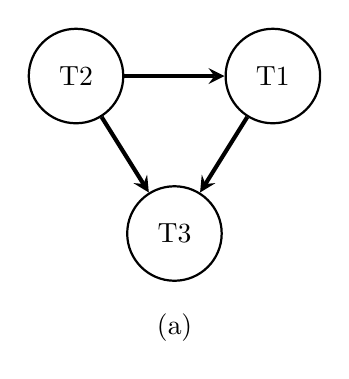
\begin{tikzpicture}[node distance=3cm, >=stealth, thick]
\node[draw, circle, minimum size=1.2cm] (T2) at (0,0) {T2};
\node[draw, circle, minimum size=1.2cm] (T1) at (2.5,0) {T1};
\node[draw, circle, minimum size=1.2cm] (T3) at (1.25,-2) {T3};
\draw[->, line width=1.5pt] (T2) -- (T1);
\draw[->, line width=1.5pt] (T1) -- (T3);
\draw[->, line width=1.5pt] (T2) -- (T3);
\node[below of=T3, node distance=1.2cm] {(a)};
\end{tikzpicture}
\end{center}

\begin{center}
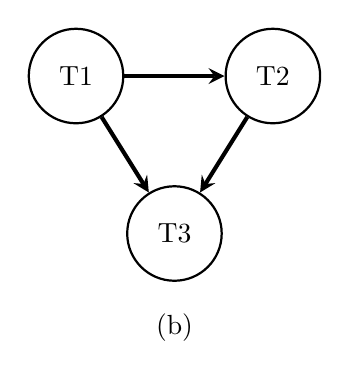
\begin{tikzpicture}[node distance=3cm, >=stealth, thick]
\node[draw, circle, minimum size=1.2cm] (T1) at (0,0) {T1};
\node[draw, circle, minimum size=1.2cm] (T2) at (2.5,0) {T2};
\node[draw, circle, minimum size=1.2cm] (T3) at (1.25,-2) {T3};
\draw[->, line width=1.5pt] (T1) -- (T2);
\draw[->, line width=1.5pt] (T1) -- (T3);
\draw[->, line width=1.5pt] (T2) -- (T3);
\node[below of=T3, node distance=1.2cm] {(b)};
\end{tikzpicture}
\end{center}

\begin{center}
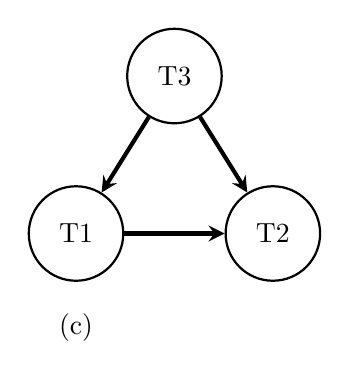
\begin{tikzpicture}[node distance=3cm, >=stealth, thick]
\node[draw, circle, minimum size=1.2cm] (T3) at (1.25,0) {T3};
\node[draw, circle, minimum size=1.2cm] (T1) at (0,-2) {T1};
\node[draw, circle, minimum size=1.2cm] (T2) at (2.5,-2) {T2};
\draw[->, line width=1.5pt] (T1) -- (T2);
\draw[->, line width=1.5pt] (T3) -- (T1);
\draw[->, line width=1.5pt] (T3) -- (T2);
\node[below of=T1, node distance=1.2cm] {(c)};
\end{tikzpicture}
\end{center}

\begin{center}
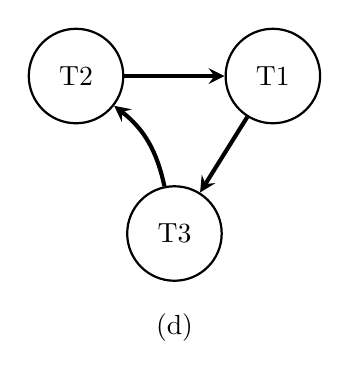
\begin{tikzpicture}[node distance=3cm, >=stealth, thick]
\node[draw, circle, minimum size=1.2cm] (T2) at (0,0) {T2};
\node[draw, circle, minimum size=1.2cm] (T1) at (2.5,0) {T1};
\node[draw, circle, minimum size=1.2cm] (T3) at (1.25,-2) {T3};
\draw[->, line width=1.5pt] (T2) -- (T1);
\draw[->, line width=1.5pt] (T1) -- (T3);
\draw[->, line width=1.5pt] (T3) to [bend right=20] (T2);
\node[below of=T3, node distance=1.2cm] {(d)};
\end{tikzpicture}
\end{center}

(e) None of the above

\subsubsection{(4 points)}
Which of the following statements about Schedule (1) is \textbf{correct}? Choose \textbf{one or more} options:

(a) Schedule (1) is a serial schedule.

(b) Schedule (1) is a conflict serializable schedule.

(c) Schedule (1) is a serializable schedule.

(d) The equivalent serial schedule of Schedule (1) can be T2, T1, T3.

(e) The equivalent serial schedule of Schedule (1) can be T1, T2, T3.

(f) None of the above

\subsubsection{(3 points)}
Analyze Schedule (2). Which type(s) of schedule does Schedule (2) belong to? Choose \textbf{one or more} options:

(a) Serial schedule

(b) Serializable schedule

(c) Conflict serializable schedule

(d) None of the above

\newpage
\newpage

% ============================================================================
% ANSWERS SECTION
% ============================================================================

\section*{ANSWERS SECTION}

\hrule
\vspace{1em}

\subsection*{Question 1: Relational Algebra}

\subsubsection*{1.1 (4 points)}
\textcolor{red}{\textbf{Box 1:} pi (projection)}

\textcolor{red}{\textbf{Box 2:} sigma (selection)}

\textcolor{red}{\textbf{Box 3:} sigma (selection)}

\textcolor{red}{\textbf{Box 4:} studio}

\textcolor{red}{\textbf{Complete answer:} $\Pi_{\text{uid, username}}(\sigma_{\text{rating} = 5}(\text{subscriber} \bowtie \text{viewing} \bowtie \text{movie} \bowtie (\sigma_{\text{country = 'USA'}}(\text{studio}))))$}

\textcolor{red}{\textbf{Explanation:} Join all tables to connect subscribers to studios through viewings and movies, then filter for USA studios with rating = 5, and project the required attributes.}

\subsubsection*{1.2 (6 points)}
\textcolor{red}{\textbf{Box 5:} subscriber}

\textcolor{red}{\textbf{Box 6:} - (minus / set difference)}

\textcolor{red}{\textbf{Box 7:} sigma (selection)}

\textcolor{red}{\textbf{Box 8:} movie}

\textcolor{red}{\textbf{Complete answer:} $\Pi_{\text{uid}}(\text{subscriber}) - \Pi_{\text{uid}}(\text{viewing} \bowtie_{\text{viewing.mid = movie.mid}} (\sigma_{\text{genre = 'Horror'}}(\text{movie})))$}

\textcolor{red}{\textbf{Explanation:} All subscriber UIDs MINUS those who have watched Horror movies = subscribers who have NOT watched any Horror movie. This is the standard ``NOT'' pattern in relational algebra.}

\hrule
\vspace{1em}

\subsection*{Question 2: SQL}

\subsubsection*{2.1.1 (2 points)}
\textcolor{red}{\textbf{Answer: (b) False}}

\textcolor{red}{Any comparison with NULL (including NULL = NULL) yields UNKNOWN, not TRUE. To check for NULL, you must use IS NULL or IS NOT NULL.}

\subsubsection*{2.1.2 (2 points)}
\textcolor{red}{\textbf{Answer: (a) True}}

\textcolor{red}{x IN (empty set) is FALSE because x cannot be equal to any element in an empty set. x > ALL (empty set) is TRUE (vacuously true) because x is greater than all zero values in the empty set.}

\subsubsection*{2.2.1 (4 points)}
\textcolor{red}{\textbf{Answer: (b)}}

\textcolor{red}{Option (b) correctly joins viewing and movie on mid and groups by genre. Option (a) is wrong because it creates a Cartesian product without proper join condition. Option (c) is wrong because viewing doesn't have a genre column. Option (d) has invalid syntax.}

\subsubsection*{2.2.2 (4 points)}
\textcolor{red}{\textbf{Answer: (b)}}

\textcolor{red}{Correct: GROUP BY uid, then HAVING COUNT(*) > 10 filters groups. Cannot use aggregate functions like COUNT in WHERE clause (option a). Option (c) uses non-aggregated mid in HAVING. Option (d) is missing GROUP BY.}

\subsubsection*{2.2.3 (4 points)}
\textcolor{red}{\textbf{Box 1:} EXISTS}

\textcolor{red}{\textbf{Box 2:} AND}

\textcolor{red}{\textbf{Complete query:}}
\begin{verbatim}
SELECT DISTINCT s.sid, s.studioName
FROM studio s
WHERE EXISTS (
    SELECT * FROM movie m
    WHERE m.sid = s.sid AND m.genre = 'Action'
);
\end{verbatim}

\textcolor{red}{\textbf{Explanation:} EXISTS checks if the correlated subquery returns at least one row. For each studio, we check if there exists a movie record with matching sid and genre = 'Action'.}

\subsubsection*{2.2.4 (4 points)}
\textcolor{red}{\textbf{Answer: (f) All of the above}}

\textcolor{red}{(a) TRUE: LEFT JOIN preserves all subscribers. (b) TRUE: WHERE v.uid IS NULL filters for those without viewings. (c) TRUE: equivalent to NOT IN approach. (d) TRUE: INNER JOIN only returns matching rows, but then filtering for IS NULL means no rows match (empty result). (e) TRUE: IS NULL checks for no matching records.}

\hrule
\vspace{1em}

\subsection*{Question 3: ER Modeling}

\subsubsection*{3.1.1 (2 points)}
\textcolor{red}{\textbf{Answer: (a) True}}

\textcolor{red}{A weak entity type IS represented by a double-bordered rectangle, and its identifying relationship (the relationship that connects it to its owner entity) IS represented by a double-bordered diamond. This is standard ER notation.}

\subsubsection*{3.1.2 (2 points)}
\textcolor{red}{\textbf{Answer: (b) False}}

\textcolor{red}{In a 1:N relationship, the foreign key is placed on the N-side (the ``many'' side), NOT the ``one'' side. This is because each entity on the N-side references exactly one entity on the 1-side. Placing the FK on the 1-side would require storing multiple values (violating 1NF).}

\subsubsection*{3.1.3 (2 points)}
\textcolor{red}{\textbf{Answer: (a) True}}

\textcolor{red}{Composite attributes (e.g., ``address'' with components street, city, zip) are flattened to their simple components when mapping to the relational model. Only the leaf-level simple attributes are stored; the composite grouping itself is not represented as a column.}

\subsubsection*{3.2 (4 points)}
\textcolor{red}{\textbf{Answer: (a)}}

\textcolor{red}{\textbf{Interpretation of the requirements:}}
\textcolor{red}{\begin{itemize}
\item Guest [1,*]: must reserve (min=1, total participation shown by double line) at least one room (max=*)
\item Room [0,*]: can be reserved by none (min=0, partial participation) or many guests (max=*)
\item Chen notation: M near guest (many guests), N near room (many rooms) - this is M:N
\end{itemize}}

\textcolor{red}{\textbf{Why other options are wrong:}}
\textcolor{red}{\begin{itemize}
\item (b): Participation swapped - would mean rooms must be reserved (total) and guests are optional (partial)
\item (c): Shows N:1 relationship where guest reserves exactly one room [1,1] - wrong cardinality
\item (d): Participation completely swapped between entities
\end{itemize}}

\subsubsection*{3.3 (6 points)}
\textcolor{red}{\textbf{Answer: (b), (c), (e)}}

\textcolor{red}{\textbf{Correct mapping (3 relations):}}
\textcolor{red}{\begin{itemize}
\item \textbf{(b)} album(\underline{albumID}, title)
  \begin{itemize}
  \item Strong entity with simple attributes only
  \item genre is multi-valued $\rightarrow$ separate table (NOT included here)
  \end{itemize}
\item \textbf{(c)} genre(\underline{albumID $\rightarrow$ album, genreName})
  \begin{itemize}
  \item Multi-valued attribute creates separate table
  \item Composite PK: albumID + genreName (both underlined)
  \end{itemize}
\item \textbf{(e)} song(\underline{albumID $\rightarrow$ album, trackNo}, title, duration)
  \begin{itemize}
  \item Weak entity mapping: owner's PK (albumID) + partial key (trackNo) = composite PK
  \item albumID is both FK and part of PK
  \item All simple attributes of song included
  \end{itemize}
\end{itemize}}

\textcolor{red}{\textbf{Why other options are wrong:}}
\textcolor{red}{\begin{itemize}
\item (a): genre should NOT be in album table (it's multi-valued)
\item (d): trackNo alone cannot be PK for weak entity (needs owner's PK too)
\item (f): No separate ``contains'' table needed - weak entity absorbs the identifying relationship
\item (g): Weak entities don't get their own independent ID; they use owner's PK + partial key
\end{itemize}}

\hrule
\vspace{1em}

\subsection*{Question 4: Design Theory}

\subsubsection*{4.1.1 (2 points)}
\textcolor{red}{\textbf{Answer: (a) True}}

\textcolor{red}{Armstrong's axiom of transitivity states: If $X \rightarrow Y$ and $Y \rightarrow Z$, then $X \rightarrow Z$. This is one of the three fundamental axioms (Reflexivity, Augmentation, Transitivity) that form the basis for deriving all valid functional dependencies.}

\subsubsection*{4.1.2 (2 points)}
\textcolor{red}{\textbf{Answer: (a) True}}

\textcolor{red}{This is the exact definition of BCNF. A relation is in BCNF if and only if for every non-trivial FD $X \rightarrow Y$, the left-hand side $X$ is a superkey. Unlike 3NF, BCNF has no exception for prime attributes on the RHS.}

\subsubsection*{4.2.1 (4 points)}
\textcolor{red}{\textbf{Answer: (c), (d), (e), (f)}}

\textcolor{red}{First, identify that C never appears on RHS of any FD, so C must be in every candidate key.}

\textcolor{red}{Computing closures:}
\textcolor{red}{\begin{itemize}
\item $(AC)^+ = \{A, C, B, D, E\}$ (using $A \rightarrow B$, $BC \rightarrow D$, $D \rightarrow E$) - \textbf{candidate key!}
\item $(BC)^+ = \{B, C, D, E, A\}$ (using $BC \rightarrow D$, $D \rightarrow E$, $E \rightarrow A$) - \textbf{candidate key!}
\item $(DC)^+ = \{D, C, E, A, B\}$ (using $D \rightarrow E$, $E \rightarrow A$, $A \rightarrow B$) - \textbf{candidate key!}
\item $(EC)^+ = \{E, C, A, B, D\}$ (using $E \rightarrow A$, $A \rightarrow B$, $BC \rightarrow D$) - \textbf{candidate key!}
\item A alone: $A^+ = \{A, B\}$ - not a superkey (missing C, D, E)
\item C alone: $C^+ = \{C\}$ - not a superkey
\item ABC is a superset of AC, so it's a superkey but NOT minimal (not a candidate key)
\end{itemize}}

\subsubsection*{4.2.2 (3 points)}
\textcolor{red}{\textbf{Answer: (b) 3NF but not BCNF}}

\textcolor{red}{Candidate keys: AC, BC, DC, EC. Prime attributes: A, B, C, D, E (ALL are prime!)}

\textcolor{red}{Check BCNF: For $A \rightarrow B$, A is not a superkey ($A^+ = \{A, B\}$). Violates BCNF.}

\textcolor{red}{Check 3NF: For each FD, either LHS is superkey OR RHS is prime:}
\textcolor{red}{\begin{itemize}
\item $A \rightarrow B$: A not superkey, but B is prime (part of key BC) \checkmark
\item $BC \rightarrow D$: BC is superkey \checkmark
\item $D \rightarrow E$: D not superkey, but E is prime (part of key EC) \checkmark
\item $E \rightarrow A$: E not superkey, but A is prime (part of key AC) \checkmark
\end{itemize}}
\textcolor{red}{All FDs satisfy 3NF condition, so relation is in 3NF but not BCNF.}

\subsubsection*{4.2.3 (3 points)}
\textcolor{red}{\textbf{Answer: (b), (c)}}

\textcolor{red}{For lossless decomposition: $(R_1 \cap R_2)^+$ must contain $(R_1 - R_2)$ or $(R_2 - R_1)$.}

\textcolor{red}{(a) $R_1 \cap R_2 = \{C\}$. $C^+ = \{C\}$. Doesn't contain $\{A, B\}$ or $\{D, E\}$. \textbf{NOT lossless.}}

\textcolor{red}{(b) $R_1 \cap R_2 = \{D\}$. $D^+ = \{D, E, A, B\}$. Contains $R_1 - R_2 = \{A, B\}$! \textbf{Lossless!}}

\textcolor{red}{(c) $R_1 \cap R_2 = \{D\}$. $D^+ = \{D, E, A, B\}$. Contains $R_2 - R_1 = \{A, E\}$! \textbf{Lossless!}}

\textcolor{red}{(d) $R_1 \cap R_2 = \{B\}$. $B^+ = \{B\}$. Doesn't contain $\{A\}$ or $\{C, D, E\}$. \textbf{NOT lossless.}}

\hrule
\vspace{1em}

\subsection*{Question 5: Physical Design}

\subsubsection*{5.1.1 (2 points)}
\textcolor{red}{\textbf{Answer: (a) True}}

\textcolor{red}{In B+ trees, all data records (or pointers to data records) are stored only in the leaf nodes. Internal nodes contain only keys (used as separators/guides for navigation) and child pointers. This is the fundamental distinction between B+ trees and B-trees.}

\subsubsection*{5.1.2 (2 points)}
\textcolor{red}{\textbf{Answer: (a) True}}

\textcolor{red}{For degree $d = 5$: minimum keys in leaf = $\lceil (d-1)/2 \rceil = \lceil (5-1)/2 \rceil = \lceil 4/2 \rceil = 2$.}

\subsubsection*{5.2.1 (4 points)}
\textcolor{red}{\textbf{Answer: (c)}}

\textcolor{red}{\textbf{Step-by-step analysis:}}

\textcolor{red}{\textbf{Initial tree (d=4):} Root [15 $|$ 28] with leaves [5* 10*], [15* 20* 25*], [28* 35* 40*].}

\textcolor{red}{\textbf{For d=4:} min leaf keys = $\lceil (4-1)/2 \rceil = 2$, max leaf keys = $d-1 = 3$.}

\textcolor{red}{\textbf{Delete 5*:} Leaf becomes [10*] (1 key $<$ 2 minimum $\rightarrow$ underflow!).
Right sibling [15* 20* 25*] has 3 keys (more than minimum 2), so we can \textbf{redistribute}.
Borrow 15* from sibling: left leaf becomes [10* 15*], sibling becomes [20* 25*].
Update separator key in root: first key of new right leaf = 20.
Root becomes [20 $|$ 28].}

\textcolor{red}{\textbf{Delete 10*:} Leaf [10* 15*] becomes [15*] (1 key $<$ 2 minimum $\rightarrow$ underflow!).
Right sibling [20* 25*] has only 2 keys (exactly minimum), cannot redistribute.
Must \textbf{merge}: combine [15*] with [20* 25*] $\rightarrow$ [15* 20* 25*] (3 keys, valid).
Remove separator 20 from root. Root becomes [28] with 2 leaves.}

\textcolor{red}{\textbf{Final result:} Root [28] with leaves [15* 20* 25*] and [28* 35* 40*]. This matches option (c).}

\textcolor{red}{\textbf{Why other options are wrong:}
\begin{itemize}
\item (a) Wrong separator (15 should not be in root after merge)
\item (b) Wrong separator and structure
\item (d) Shows underflow not handled (leaf with only 1 key)
\end{itemize}}

\subsubsection*{5.2.2 (4 points)}
\textcolor{red}{\textbf{Answer: (c)}}

\textcolor{red}{\textbf{Step-by-step analysis:}}

\textcolor{red}{\textbf{Initial tree (d=4):} Root [15 $|$ 28] with leaves [5* 10*], [15* 20* 25*], [28* 35* 40*].}

\textcolor{red}{\textbf{Insert 22*:} Goes to leaf [15* 20* 25*].
After insertion: [15* 20* 22* 25*] (4 keys, but max = $d-1 = 3$ $\rightarrow$ overflow!)}

\textcolor{red}{\textbf{Split leaf:}
\begin{itemize}
\item Left leaf gets $\lfloor 4/2 \rfloor = 2$ keys: [15* 20*]
\item Right leaf gets $\lceil 4/2 \rceil = 2$ keys: [22* 25*]
\item \textbf{Copy up} first key of right leaf = 22
\end{itemize}}

\textcolor{red}{\textbf{Update parent:} Insert key 22 into root [15 $|$ 28].
Root becomes [15 $|$ 22 $|$ 28] with 4 children (valid for d=4, max children = 4).}

\textcolor{red}{\textbf{Final result:} Root [15 $|$ 22 $|$ 28] with leaves:
[5* 10*], [15* 20*], [22* 25*], [28* 35* 40*]. This matches option (c).}

\hrule
\vspace{1em}

\subsection*{Question 6: Query Processing and Optimization}

\subsubsection*{6.1.1 (2 points)}
\textcolor{red}{\textbf{Answer: (a) True}}

\textcolor{red}{This statement correctly describes 2-Way External Merge Sort:}
\textcolor{red}{\begin{itemize}
\item Phase 1: Read $B$ pages into memory, sort them, write out a sorted run of size $B$ pages
\item Phase 2: Merge exactly 2 runs at a time (regardless of how many buffers are available)
\item This is why it's called ``2-Way'' -- it only merges 2 runs per pass
\end{itemize}}

\subsubsection*{6.1.2 (2 points)}
\textcolor{red}{\textbf{Answer: (a) True}}

\textcolor{red}{In Multi-Way External Merge Sort with $B$ buffer pages:}
\textcolor{red}{\begin{itemize}
\item We need 1 buffer page for output
\item The remaining $B-1$ buffer pages can each hold one page from a different run
\item Therefore, we can merge up to $B-1$ runs simultaneously in each pass
\end{itemize}}

\subsubsection*{6.2.1 (4 points)}
\textcolor{red}{\textbf{Answer: (a), (b), (c), (d), (e)}}

\textcolor{red}{\textbf{Given:} 90,000 tuples, 50 tuples/page, 100 buffer pages}

\textcolor{red}{(a) Pages for $R$: $90,000 / 50 = 1,800$ pages. \textbf{Correct!}}

\textcolor{red}{(b) Phase 1 runs: $\lceil 1,800 / 100 \rceil = 18$ runs. \textbf{Correct!}}

\textcolor{red}{(c) Phase 2: With 100 buffers, we can merge $100-1=99$ runs per pass. Since $18 < 99$, we need only 1 pass. \textbf{Correct!}}

\textcolor{red}{(d) Total I/O = $2 \times \text{pages} \times (1 + \text{Phase 2 passes})$}
\textcolor{red}{$= 2 \times 1,800 \times (1 + 1) = 7,200$ page transfers. \textbf{Correct!}}

\textcolor{red}{(e) With 10 buffers: $\lceil 1,800 / 10 \rceil = 180$ runs. \textbf{Correct!}}

\subsubsection*{6.2.2 (2 points)}
\textcolor{red}{\textbf{Answer: (a)}}

\textcolor{red}{2-Way External Merge Sort Phase 2 passes formula: $\lceil \log_2 N_0 \rceil$}
\textcolor{red}{where $N_0$ = number of initial sorted runs = number of pages (in 2-Way, each page becomes one initial run)}

\textcolor{red}{$\lceil \log_2 1,800 \rceil = 11$ passes (since $2^{10} = 1024 < 1800$ and $2^{11} = 2048 > 1800$)}

\subsubsection*{6.3 (4 points)}
\textcolor{red}{\textbf{Answer: (a), (b), (c), (d), (e)}}

\textcolor{red}{\textbf{Given:} $|S| = 4,000$ pages, $|T| = 200$ pages, $B = 52$ buffers}

\textcolor{red}{\textbf{Block Nested-Loop Join formula:} Cost = $|outer| + \lceil |outer|/(B-2) \rceil \times |inner|$}

\textcolor{red}{(a) $T$ as outer: $200 + \lceil 200/50 \rceil \times 4,000 = 200 + 4 \times 4,000 = 16,200$. \textbf{Correct!}}

\textcolor{red}{(b) $S$ as outer: $4,000 + \lceil 4,000/50 \rceil \times 200 = 4,000 + 80 \times 200 = 20,000$. \textbf{Correct!}}

\textcolor{red}{(c) Since $16,200 < 20,000$, using smaller relation as outer minimizes I/O. \textbf{Correct!}}

\textcolor{red}{(d) $\lceil 200/50 \rceil = 4$ iterations when $T$ is outer. \textbf{Correct!}}

\textcolor{red}{(e) The formula is correct. \textbf{Correct!}}

\hrule
\vspace{1em}

\subsection*{Question 7: Transactions, Concurrency Control, and Recovery}

\subsubsection*{7.1.1 (2 points)}
\textcolor{red}{\textbf{Answer: (a) True}}

\textcolor{red}{REDO processes log forward (beginning to end) to reapply committed changes.}

\subsubsection*{7.1.2 (2 points)}
\textcolor{red}{\textbf{Answer: (a) True}}

\textcolor{red}{Deadlock occurs when transactions form a cycle in the wait-for graph, each waiting for locks held by others.}

\subsubsection*{7.2.1 (3 points)}
\textcolor{red}{\textbf{Answer: (a)}}

\textcolor{red}{Conflicts in Schedule (1):}
\textcolor{red}{\begin{itemize}
\item T2: W(M) before T1: R(M) $\rightarrow$ T2 $\rightarrow$ T1
\item T1: W(N) before T3: R(N) $\rightarrow$ T1 $\rightarrow$ T3
\item T2: W(P) before T3: R(P) $\rightarrow$ T2 $\rightarrow$ T3
\end{itemize}}

\textcolor{red}{Graph: T2 $\rightarrow$ T1, T1 $\rightarrow$ T3, T2 $\rightarrow$ T3}

\subsubsection*{7.2.2 (4 points)}
\textcolor{red}{\textbf{Answer: (b), (c), (d)}}

\textcolor{red}{(b) Acyclic precedence graph means conflict serializable. \textbf{True!}}

\textcolor{red}{(c) All conflict serializable schedules are serializable. \textbf{True!}}

\textcolor{red}{(d) Topological sort gives: T2, T1, T3. \textbf{True!}}

\subsubsection*{7.2.3 (3 points)}
\textcolor{red}{\textbf{Answer: (b), (c)}}

\textcolor{red}{Conflicts in Schedule (2):}
\textcolor{red}{\begin{itemize}
\item T1: R(M) before T2: W(M) $\rightarrow$ T1 $\rightarrow$ T2
\item T2: W(M) before T3: W(M) $\rightarrow$ T2 $\rightarrow$ T3
\item T1: W(N) before T3: R(N) $\rightarrow$ T1 $\rightarrow$ T3
\item T2: W(P) before T3: R(P) $\rightarrow$ T2 $\rightarrow$ T3
\end{itemize}}

\textcolor{red}{The precedence graph is: T1 $\rightarrow$ T2, T2 $\rightarrow$ T3, T1 $\rightarrow$ T3.}

\textcolor{red}{This is acyclic! So it IS conflict serializable and serializable. Equivalent serial order: T1, T2, T3.}

\end{document}
